\documentclass[twocolumn]{autart}

\usepackage{graphicx}
\usepackage{algpseudocode}
\usepackage{url}

\begin{document}

\begin{frontmatter}

\title{A Lightweight Networking Strategy for Robotic Control Systems\thanksref{footnoteinfo}}

\thanks[footnoteinfo]{This paper was not presented at any IFAC meeting. Corresponding author N.~S.~Selby.}

\author[MIT]{Jake Robert Read\thanksref{equalAuth}}\ead{jake.read@cba.mit.edu},
\author[Ethiopia]{Nicholas Stearns Selby\thanksref{equalAuth}}\ead{nicholas.selby@renewvia.com},\author[Patrick]{Patrick Wahl}\ead{pwahl@alum.mit.edu},
\author[Doug]{Douglas Kogut}\ead{dkogut@alum.mit.edu}

\thanks[equalAuth]{Authors Jake Robert Read and Nicholas Stearns Selby contributed equally to this work.}

\address[Ethiopia]{Renewvia Solar Ethiopia PLC, Addis Ababa, Ethiopia, Bole sub-city, Woreda 03, House No. 174/175, Saya Building, 5th Floor}
\address[MIT]{The MIT Center for Bits and Atoms, Room E15-401, 20 Ames Street, Cambridge, MA 02139}
\address[Patrick]{210 Green Street, Cambridge, MA 02139}
\address[Doug]{77 Massachusetts Avenue, Cambridge, MA 02139}
		  
\begin{keyword} % 5-10 chosend from IFAC keyword list
	Networked control systems; Control of networks; networked robotics; computer networks; fault-tolerant
\end{keyword}


\begin{abstract}    % Word limit: 200
	We introduce TinyNet, an innovative open-source networking protocol tailored for Networked Control Systems, designed to be easily implementable on system endpoints with minimal complexity. Distinguished by its operation without a global state, TinyNet enhances memory efficiency and fault tolerance. It facilitates real-time multipath routing through a local table at each router, identifying the shortest path for each destination node via each router's ports. A key feature of TinyNet is its utilization of a ``busyness-metric'' based cost function, which considers the buffer size at each neighbor node. This approach effectively prevents routing bottlenecks and maximizes network utilization. TinyNet's design focuses on transmitting small packet sizes, optimizing data transmission efficiency. This makes it particularly suitable for streamlined network models, especially those primarily concerned with sustaining control loops. Performance evaluations demonstrate that TinyNet achieves notable improvements in message delivery time determinism and robustness against network failures, making it a promising solution for distributed robotic control systems.
\end{abstract}

\end{frontmatter}

\section{Introduction}
Networked control systems (NCS) are integral components of sophisticated robotics and avionics, orchestrating the collaborative function of numerous sensors and actuators to achieve objectives such as locomotion, stabilization, sensor fusion, and position control \cite{gupta2009networked,moyne2007emergence}. Additionally, NCS play a pivotal role in manufacturing settings, interlinking multiple machines for synchronized material handling and production planning \cite{vitturi2019industrial}. This field distinguishes itself from conventional networking paradigms in several key aspects:

\begin{enumerate}
    \item \textbf{Prioritization of Message Efficiency Over Throughput:} Unlike traditional networks where throughput is paramount, NCS prioritize efficient message sizes, typically ranging from three to fifty bytes \cite{gupta2009networked}. The emphasis is on the rapidity of message delivery, with many communications comprising single-packet messages.
    \item \textbf{Critical Need for Deterministic Message Delivery:} In NCS, the stability of control loops is contingent upon the guarantee of message delivery within specific time frames \cite{moyne2007emergence}. This necessitates a network where the round trip times (RTTs) have minimal variability, ensuring reliable and predictable communication.
    \item \textbf{Essential Robustness and Simplified Management:} Robustness in NCS is non-negotiable, requiring the absence of single points of failure \cite{vitturi2019industrial}. Furthermore, these systems are designed to operate independently of network controllers for coordinating port-forwarding configurations. Avoiding central management for route adjustments on all nodes is crucial, as it significantly reduces complexities and variations in RTTs.
\end{enumerate}

In summary, NCS demand a unique networking approach focused on small, swift message exchanges, determinism in delivery times, and a robust, decentralized architecture to maintain system stability and efficiency.

Recent developments in the field of NCS have seen a gradual shift from traditional fieldbuses to more contemporary networking solutions. Currently, the state-of-the-art in NCS predominantly involves the use of Switched Ethernet or its derivatives in proprietary protocols \cite{gupta2009networked,moyne2007emergence}. This transition has been driven by the greater accessibility of Switched Ethernet hardware and its status as an open standard. Such features facilitate the integration of control products from various vendors, enabling customers to build more scalable and complex systems without the need for extensive reconfiguration or adherence to FieldBus specifications.

Despite its widespread adoption, Switched Ethernet falls short in addressing the specialized requirements of NCS. Its design, primarily tailored for general-purpose networking, does not align perfectly with the unique needs of NCS, particularly in areas such as real-time data transmission and network robustness. In Section~\ref{sec:related}, we discuss a key limitation of Switched Ethernet: its inability to support more than one route to any given endpoint in a network graph. This constraint leads to bottlenecks at specific switches and introduces Single Points of Failure (SPoF) in network architectures. Consequently, a failure in a single link can render many endpoints irreversibly inaccessible.

To enhance Message Delivery Determinism, a key performance indicator for NCS, we propose the implementation of a multipath routing strategy. This approach allows for the operation of NCS within highly interconnected graph structures, as opposed to limited spanning-tree configurations. It enables the rerouting of messages around congested nodes instead of accumulating them in extensive buffers.

However, current multipath routing methods, predominantly designed for datacenter environments, rely heavily on network controllers (NCs) to manage and update port-forwarding tables. These NCs hold comprehensive information about the entire network's state. In scenarios like a link failure or a sudden surge in network traffic (for instance, due to a router becoming overloaded), these controllers must reconverge to a new suitable routing topology and disseminate updated routing instructions across the network. This reconvergence takes as little as 50~ms with modern Fast Reroute pre-computation~\cite{cisco_lfa} and up to several hundred milliseconds with vanilla link-state protocols~\cite{eramo2008multi,farkas2009performance}. Such delays, albeit brief, can disrupt the entire network operation temporarily, leading to potential failures in the control loops of an NCS. Therefore, these existing multipath routing methods, given their reliance on network controller-based reconvergence, are not ideally suited for application in NCS.

Taken together, the limitations identified above---single points of failure, spanning-tree bottlenecks, and controller-dependent reconvergence delays---motivate the design of a stateless, multipath routing protocol purpose-built for NCS. To the authors' knowledge, TinyNet is the first protocol to combine the simplicity of Switched Ethernet with the multipath routing benefits found in datacenter networks, without requiring a central controller. It enables multipath capabilities without relying on a network controller for managing forwarding tables, achieved through a port-forwarding algorithm that utilizes each router's \textit{local awareness} of neighboring nodes' packet queues and historical data on packet transmissions observed at the router's ports. We describe the protocol rules and evaluate performance through hardware experiments and simulation.
\section{Related Work}
\label{sec:related}
 
TinyNet sits at the intersection of several mature research and engineering communities: deterministic industrial Ethernet, IP-layer fast reroute, congestion-aware multipath in datacenter fabrics, backpressure-based routing for multi-hop wireless networks, and mesh routing for constrained devices. We survey each in turn, identifying the specific gap that motivates a stateless,busyness-aware protocol for networked control.
 
\subsection{Deterministic Industrial Ethernet}
\label{sec:related:industrial}
 
The dominant deployed alternatives to Switched Ethernet in NCS are the modified-Ethernet fieldbusses: EtherCAT, PROFINET~IRT, SERCOS~III, POWERLINK, and CC-Link~IE~TSN, together with the avionics-grade AFDX family. \cite{felser2005realtime,zunino2018industrial} EtherCAT, in particular, is widely used in industrial robotics and achieves sub-microsecond synchronization and cycle times below 100~$\mu$s by processing frames \emph{on the fly}: a single frame circulates around a logical ring, and each slave extracts and inserts its data as the frame passes through dedicated hardware. \cite{ethercat_ig,prytz2008performance} Reported jitter for ARM-based EtherCAT masters in robotic motion control is below 1~$\mu$s~\cite{ethercat_arm_robot}. AFDX, the deterministic Ethernet profile flying on the A350 and 787, provides bounded latency through statically allocated Virtual Links and dual redundant networks. \cite{afdx_nasa}
 
These protocols achieve excellent determinism, but at a cost that TinyNet is explicitly designed to avoid. EtherCAT requires a master to own the cycle and constrains the topology to ring or line structures; AFDX statically provisions every Virtual Link offline, requires certified switch hardware, and uses redundancy rather than multipath (the two copies follow disjoint but fixed paths). Neither addresses the case of a richly meshed graph of peer endpoints discovering routes at runtime without a controller.
 
The IEEE 802.1 Time-Sensitive Networking (TSN) family of standards augments standard switched Ethernet with deterministic mechanisms and is now widely deployed in industrial automation, automotive, and aerospace settings. \cite{tsn_survey_arxiv,tsn_ieee_tg} In particular, the 802.1Qcc enhancement defines fully centralized, fully distributed, and hybrid models for configuring TSN networks. \cite{nasrallah_qcc_arxiv}
 
Two TSN features are directly comparable to TinyNet's claims and deserve closer attention than they have received in the NCS literature. First, FRER addresses fault tolerance by transmitting duplicated frames over a network, which may include disjoint paths, and eliminating duplicates at the receiver; this is a different point in the design space than TinyNet's reactive flooding, but it accomplishes a similar goal without paying the cost of post-failure reconvergence. Second, TAS (802.1Qbv) achieves bounded jitter by computing a global gate schedule offline, an approach whose schedulability problem is NP-complete and which has spawned a large literature on SMT-based and heuristic synthesis. \cite{craciunas2016combined,tsnsched,tsn_scheduling_survey} TAS provides excellent determinism for traffic whose timing is known at design time, but reconfiguring the schedule in response to runtime conditions remains costly, and the schedule itself is typically computed by a Centralized Network Configuration entity. TinyNet targets the complementary regime: irregular, topology-changing networks where offline scheduling is impractical and where the cost of a centralized configuration entity is unacceptable.
 
\subsection{IP-Layer Fast Reroute}
\label{sec:related:frr}
 
The 200~ms reconvergence figure cited for OSPF and SPB \cite{ospf,spb} reflects the behavior of vanilla link-state protocols and was the relevant baseline at the time those measurements were taken. Modern IP networks largely avoid this latency through pre-computed local repair. Loop-Free Alternates (LFA~\cite{rfc5286}), Remote-LFA, and Topology-Independent LFA install a backup next-hop in the forwarding table at routing-protocol convergence time; when Bidirectional Forwarding Detection or a link-down signal triggers failover, the cutover is local and is typically completed in under 50ms \cite{cisco_lfa}. MPLS Fast Reroute provides comparable guarantees in MPLS-TE networks.
 
These mechanisms reduce the gap between stateful and stateless recovery from two orders of magnitude to roughly one. They do not eliminate it: LFA computes alternates against a single failure assumption, coverage is topology-dependent (not every prefix admits a loop-free alternate), and configuration complexity grows with SRLG (shared risk link group) constraints. For NCS, where control loops may run at kilohertz rates and a 50~ms blackout still corresponds to tens or hundreds of missed deadlines, these improvements are valuable, but do not close the case.
 
\subsection{Congestion-Aware Multipath in Datacenters}
\label{sec:related:dcn}
 
The datacenter networking community has produced a rich family of congestion-aware multipath schemes that are relevant to TinyNet's cost-function routing. ECMP~\cite{ecmp_rfc} splits traffic across equal-cost paths but is oblivious to congestion. CONGA~\cite{conga_sigcomm}, implemented in custom ASICs, uses leaf-switch state plus piggybacked feedback from remote leaves to make flowlet-level path decisions and reacts to congestion on the order of microseconds. Hula~\cite{hula_sosr} pushes this idea further by having each switch track only the best path to each destination through each neighbor, using probe packets in the data plane and running on programmable (P4) hardware. Other proposals like DRILL, LetFlow, Hedera, and CONGA-Flow trade off flow-completion time, asymmetry tolerance, and reordering sensitivity.
 
TinyNet's cost function in equation (\ref{eq:cost}) is structurally similar to CONGA's path-utilization metric and to Hula's per-neighbor congestion field, but the design constraints differ in three ways. First, the granularity is per-packet rather than per-flowlet, because NCS messages are typically a single packet and the notion of a flow does not usefully apply. Second, the state at each node is reduced to a single byte per neighbor (transmit buffer depth), eliminating the per-destination tables that Jula and CONGA maintain. Third, TinyNet runs on microcontroller-grade endpoints rather than programmable switches, which forces the protocol logic into roughly a hundred lines of C rather than a P4 program. These constraints rule out direct adoption of CONGA or Hula in their published form, but the analogy clarifies that TinyNet inherits and specializes a well-established line of work.
 
\subsection{Backpressure Routing}
\label{sec:related:backpressure}
 
The cost function used in TinyNet is, viewed from a different angle, a variant of backpressure routing. The original max-weight/differential-backlog algorithm of Tassiulas and Ephremides~\cite{tassiulas1992} routes packets in the direction of the steepest negative gradient of queue backlog and is throughput-optimal under broad stability conditions. Subsequent work by Neely et al.~\cite{neely2005power,neely_book} extended the framework to time-varying wireless channels and unified it with utility-optimal control. Practical realizations include BCP, the first deployed backpressure protocol for wireless sensor networks~\cite{bcp}, DiffQ for differential-backlog congestion control~\cite{diffq}, and a body of follow-up work on link-feature variants~\cite{bp_link_features}.
 
TinyNet differs from canonical backpressure in two important ways. Pure backpressure requires a separate queue per destination at each node, which is impractical for a microcontroller serving dozens of endpoints; TinyNet collapses this to a single transmit buffer per link and a small LUT, trading off a guarantee of throughput optimality for memory efficiency. And TinyNet weights backlog against hop count via the tunable $\lambda$ parameter rather than acting on backlog alone, which avoids the well-known last-packet delay problem of pure backpressure under light loads. We position TinyNet as a backpressure-inspired heuristic engineered for the NCS operating point rather than as a throughput-optimal scheme.
 
\subsection{Mesh Routing for Constrained Devices}
\label{sec:related:mesh}
 
The IETF's RPL~\cite{rfc6550} is the closest analog to TinyNet in the constrained-device space. RPL constructs a Destination-Oriented Directed Acyclic Graph (DODAG) rooted at a sink, with each node selecting a preferred parent according to a configurable Objective Function (typically Expected Transmission Count or hop count). Like TinyNet, RPL is designed for cheap nodes with limited memory and is robust to churn. Unlike TinyNet, RPL is optimized for low-power lossy links, assumes converge-cast traffic toward a root, and inherits some of the same single-tree pathologies as Spanning Tree once the DODAG is established. Reactive variants such as P2P-RPL~\cite{rfc6997} relax the converge-cast assumption but introduce on-demand route-discovery latency that NCS cannot tolerate. The mobile ad-hoc routing protocols AODV and DSR share the same trade-off: cheap to run, but with discovery latencies in the tens to hundreds of milliseconds on first contact.
 
TinyNet's flood-on-LUT-miss behavior is reminiscent of AODV's route-request flooding and of RPL's DIO/DIS exchanges, but is specialized in two ways: floods carry payload (so the first packet to a new destination is not delayed by a separate discovery round), and floods are triggered by the absence of an LUT entry rather than by a periodic timer.
 
\subsection{Position of TinyNet}
\label{sec:related:position}
 
Across these threads, TinyNet occupies a specific point:
\begin{itemize}
  \item \textbf{Compared to industrial Ethernet} (EtherCAT, PROFINET~IRT, AFDX, TSN): TinyNet sacrifices the sub-microsecond determinism and certifiability of scheduled approaches in exchange for the ability to operate on arbitrary mesh topologies without offline configuration or a centralized configuration entity.
  \item \textbf{Compared to IP-FRR}: TinyNet's failure recovery is roughly an order of magnitude faster than LFA-based fast reroute, because the response is data-driven (next packet floods) rather than gated on backup-path pre-installation and BFD detection windows.
  \item \textbf{Compared to CONGA/Hula}: TinyNet adopts the congestion-aware multipath philosophy but reduces per-node state to a single byte per neighbor and shifts the implementation target from programmable switch ASICs to commodity microcontrollers.
  \item \textbf{Compared to backpressure}: TinyNet is a memory-frugal heuristic in the same family, with a hop-count bias to prevent backlog-driven detours under light load.
  \item \textbf{Compared to RPL/AODV}: TinyNet trades the converge-cast assumption (RPL) and the separate discovery phase (AODV) for payload-carrying floods that amortize discovery into useful transmission.
\end{itemize}
 
This combination of properties---stateless, controller-free,
multipath, busyness-aware, payload-carrying floods on
discovery---does not appear together in any of the protocols above,
and is what we evaluate in Section~\ref{sec:eval}.
\section{Theory}
The TinyNet protocol significantly reduces the need for administrative communication between nodes. Rather than exchanging detailed topological data, nodes simply send periodic heartbeats to their immediate neighbors and route packets to designated ports, rendering the protocol essentially stateless. This approach allows TinyNet to operate effectively in both standard and failure situations, adopting a distributed method where the responsibility of message transmission is shifted to neighboring nodes instead of relying on pre-defined routes. Such a mechanism not only enhances link utilization but also improves the overall effective throughput (goodput) compared to alternative protocols.

We design TinyNet with the following constraints:
\begin{itemize}
	\item \textbf{Endpoint Integration:} TinyNet is engineered for straightforward integration into robotic endpoints. Utilizing a UART link, a common peripheral in most microcontrollers, the protocol is encapsulated within a C library. This design ensures that it can be effortlessly incorporated into existing firmware setups.
	\item \textbf{Open-Source Development:} We have developed TinyNet as an open-source initiative, enabling wide applicability in the development of Network Control Systems. By avoiding the creation of a proprietary standard, we envisage TinyNet being adopted in diverse hardware environments, thereby fostering various practical implementations.
	\item \textbf{Statelessness:} A core objective in TinyNet's development is to minimize the need for centralized state awareness in routing processes. This principle not only bolsters the network's overall resilience but also obviates the necessity for a central network controller or complex network configurations.
	\item \textbf{Real-Time Multipath Capability:} A significant focus of TinyNet is to provide real-time multipath routing capabilities. This feature is crucial for efficient port-forwarding and adaptive network traffic management.
	\item \textbf{Robustness:} A fundamental requirement of TinyNet is its consistent performance even in the face of link disruptions or router failures, ensuring reliability and continuity in network operations.
\end{itemize}

TinyNet's design philosophy emphasizes simplicity, adaptability, and resilience, making it an ideal solution for modern Networked Control Systems.

\subsection{The TinyNet Algorithm}
Each node handles incoming packets as follows:
\begin{algorithmic}
	\If {the packet is not a buffer update}
		\State update the LUT using packet src. and hop count
	\EndIf
	\If {packet is standard}
		\If {I am destination}
			\State process data in packet
			\State reply with ACK
		\Else
			\State increment hop count
			\If {LUT has destination address}
				\State send packet to port which minimizes C(hops, buffer) over all ports
			\Else
				\State send packet to all ports as standard flood
			\EndIf
		\EndIf
	\ElsIf {packet is ACK}
		\If {I am destination}
			\State process acknowledgement
		\Else
			\State increment hop count
			\If {LUT has destination address}
				\State send packet to port which minimizes C(hops, buffer) over all ports
			\Else
				\State send packet to all ports as ack flood
			\EndIf
		\EndIf
	\ElsIf {packet is standard flood}
		\State remove packet dest. from LUT at that port if it exists
		\If {I have not yet seen this flood}
			\If {I am destination}
				\State process data in packet
				\State reply with ACK
			\Else
				\State increment hop count
				\If {LUT has destination address}
					\State send packet to port which minimizes C(hops, buffer) as standard packet
				\Else
					\State send packet to all ports except one from which it was received
				\EndIf
			\EndIf
		\EndIf
	\ElsIf {packet is ACK flood}
		\State remove packet dest. from LUT at that port if it exists
		\If {I am destination}
			\State process acknowledgement
		\Else
			\State increment hop count
			\If {LUT has destination address}
				\State send packet to port which minimizes C(hops, buffer) as standard ACK
			\Else
				\State send packet to all ports except one from which it was received
			\EndIf
		\EndIf
	\Else
		\State write buffer depth to LUT
	\EndIf
\end{algorithmic}

\section{Implementation}
\subsection{Hardware}
For the hardware implementation of TinyNet, we developed compact routers powered by the ATSAMS70 microcontroller from Atmel/Microchip, which operates at a core clock speed of 300~MHz. The router schematic and board file are illustrated in Figs. \ref{fig:router-schematic} and \ref{fig:router-board-file} in the appendix. While this microcontroller is capable of supporting UART transmission speeds up to 18.75 Mbps, we observed that a reduction in bitrate to 3.125 Mbps was necessary to achieve stable and reliable data transmission. At higher bitrates, the inter-byte arrival interval becomes shorter than the UART interrupt service routine latency on the ATSAMS70, causing receive buffer overruns; the 3.125 Mbps setting provides sufficient margin for the 300 MHz core to service each incoming byte interrupt before the next byte arrives.

To enhance the system's resilience to electromagnetic interference (EMI), we incorporated the ISL3177 differential driver into the UART lines. Although this measure was not strictly required for our initial testing environment, it is a prudent preparatory step toward operating TinyNet in more challenging EMI conditions, such as those found near Brushless Motor Controllers. This consideration forms a part of our agenda for future development and testing, ensuring that TinyNet remains robust and reliable in a wide range of operational settings.

\subsection{Simulation}
We implemented TinyNet's software simulation in JavaScript, running on a commodity Windows laptop. The underlying framework is adapted from Simbit, a discrete-event P2P network simulator originally designed for blockchain research~\cite{simbit}; we replaced its packet format and propagation model with the UART timing equations (equations~(\ref{eq:d})--(\ref{eq:dtx})) and defined topology as an array of adjacency lists. Each element represents the port connections of one node, allowing us to model arbitrary topologies (evaluated here on up to 16 nodes).

In the simulation, each node is represented as a ``manager.'' These managers handle incoming packets on each port, maintain their own lookup and buffer depth tables, and apply the forwarding algorithm to each incoming packet. Events are scheduled by a discrete-event simulation engine that advances the virtual clock between scheduled callbacks. We can also inject custom traffic patterns to explore TinyNet's behavior under specific conditions.
\section{Evaluation}
\label{sec:eval}
To assess the effectiveness of TinyNet, we employ our hardware testbed, focusing on accurately timing key message passing intervals and associated delays. These empirical measurements serve to calibrate and inform our simulation model. The simulation, in turn, facilitates rapid iteration across a variety of network traffic scenarios. It enables us to meticulously analyze and quantify the routing paths of messages within the network, offering a detailed insight into TinyNet's performance under different conditions. This combined approach of practical testing and simulation provides a comprehensive evaluation of TinyNet's capabilities.

\subsection{Hardware}
For our hardware evaluation, we utilized the Saleae Logic 8 Logic Analyzer to capture logic level voltages from the microcontrollers. This was crucial for monitoring the router firmware at both the application and networking layers, where pin states (high or low) are indicative of significant event occurrences.

\subsubsection{Processing Delay}
\begin{figure*}[th]
    \centering
    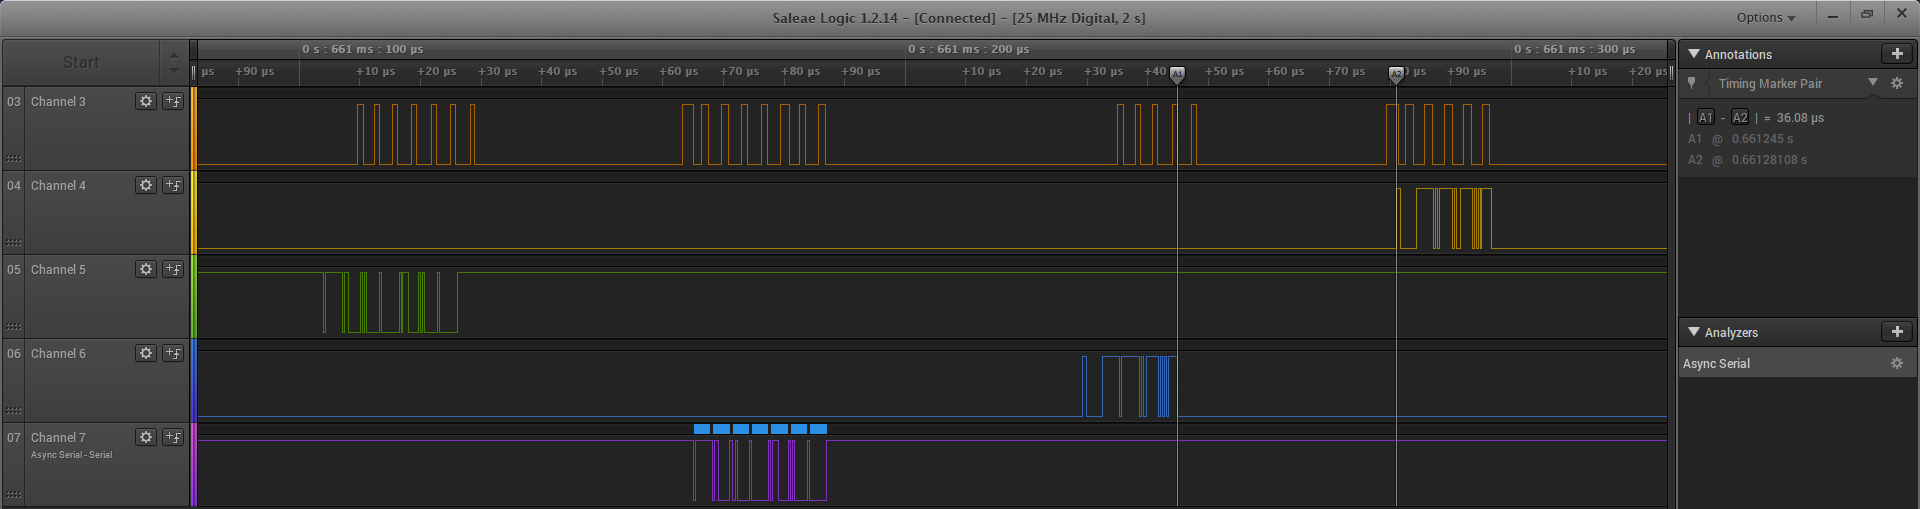
\includegraphics[width=\textwidth]{figures/results-D_p.png}
    \caption{Logic-analyzer capture showing $\mathrm{D}_{\mathrm{process}}$ measurement. Channels show UART activity: Channel 1 = incoming packet end, Channel 2 = outgoing packet start; the interval between them is $\mathrm{D}_{\mathrm{process}} = 37\,\mu\mathrm{s}$. Channel 3 shows per-byte interrupt handling ($\mathrm{D}_{\mathrm{byte}} = 1.5\,\mu\mathrm{s}$).}
    \label{fig:packet-delay}
\end{figure*}
Processing Delay, denoted $\mathrm{D}_{\mathrm{process}}$, is defined as the duration required for a router to determine the appropriate port for forwarding a received packet. To characterize this delay, we recorded signals at the link layer using the logic analyzer, tracking a packet's journey through a single router. Specifically, $\mathrm{D}_{\mathrm{process}}$ was measured as the interval between the end of an incoming packet and the start of the outgoing packet's transmission. By averaging results from 10 such packet traversals, we determined an average processing delay of $37 \mu\mathrm{s}$. The small sample size is justified by the deterministic nature of the MCU's execution path: the forwarding logic executes the same instruction sequence for every packet and runs at the exclusive priority of the main loop, with no competing interrupts during processing. Accordingly, trial-to-trial variation is negligible and the 10-sample mean is representative.

\subsubsection{Link Transmission Time}
Link Transmission Time, defined in equation~(\ref{eq:ltt}) as $\mathrm{L}_{\mathrm{tt}}$, is the time taken for a packet to travel across a link. This calculation was verified using a logic analyzer. The transmission and reception of bytes also consume processor time. As the UART link handles bit-shifting asynchronously on each port, each received character triggers an interrupt requiring processor attention. We measured this interrupt handling time to be $\mathrm{D}_{\mathrm{byte}}=1.5 \mu \mathrm{s}$ per byte, consistent across all tested packets. This value can also be derived analytically: at 300 MHz with the interrupt service routine requiring approximately 450 clock cycles for context save, buffer copy, and return, the expected handling time is $450/300\,\mathrm{MHz} = 1.5\,\mu\mathrm{s}$, confirming the measured result. This process is depicted in Fig.~\ref{fig:packet-delay}, Channel 3. We discuss in Section~\ref{sec:sim-val} how we account for these delays to align our simulation results with our hardware findings.

\subsubsection{Router Behavior}
\begin{figure}[th]
    \centering
    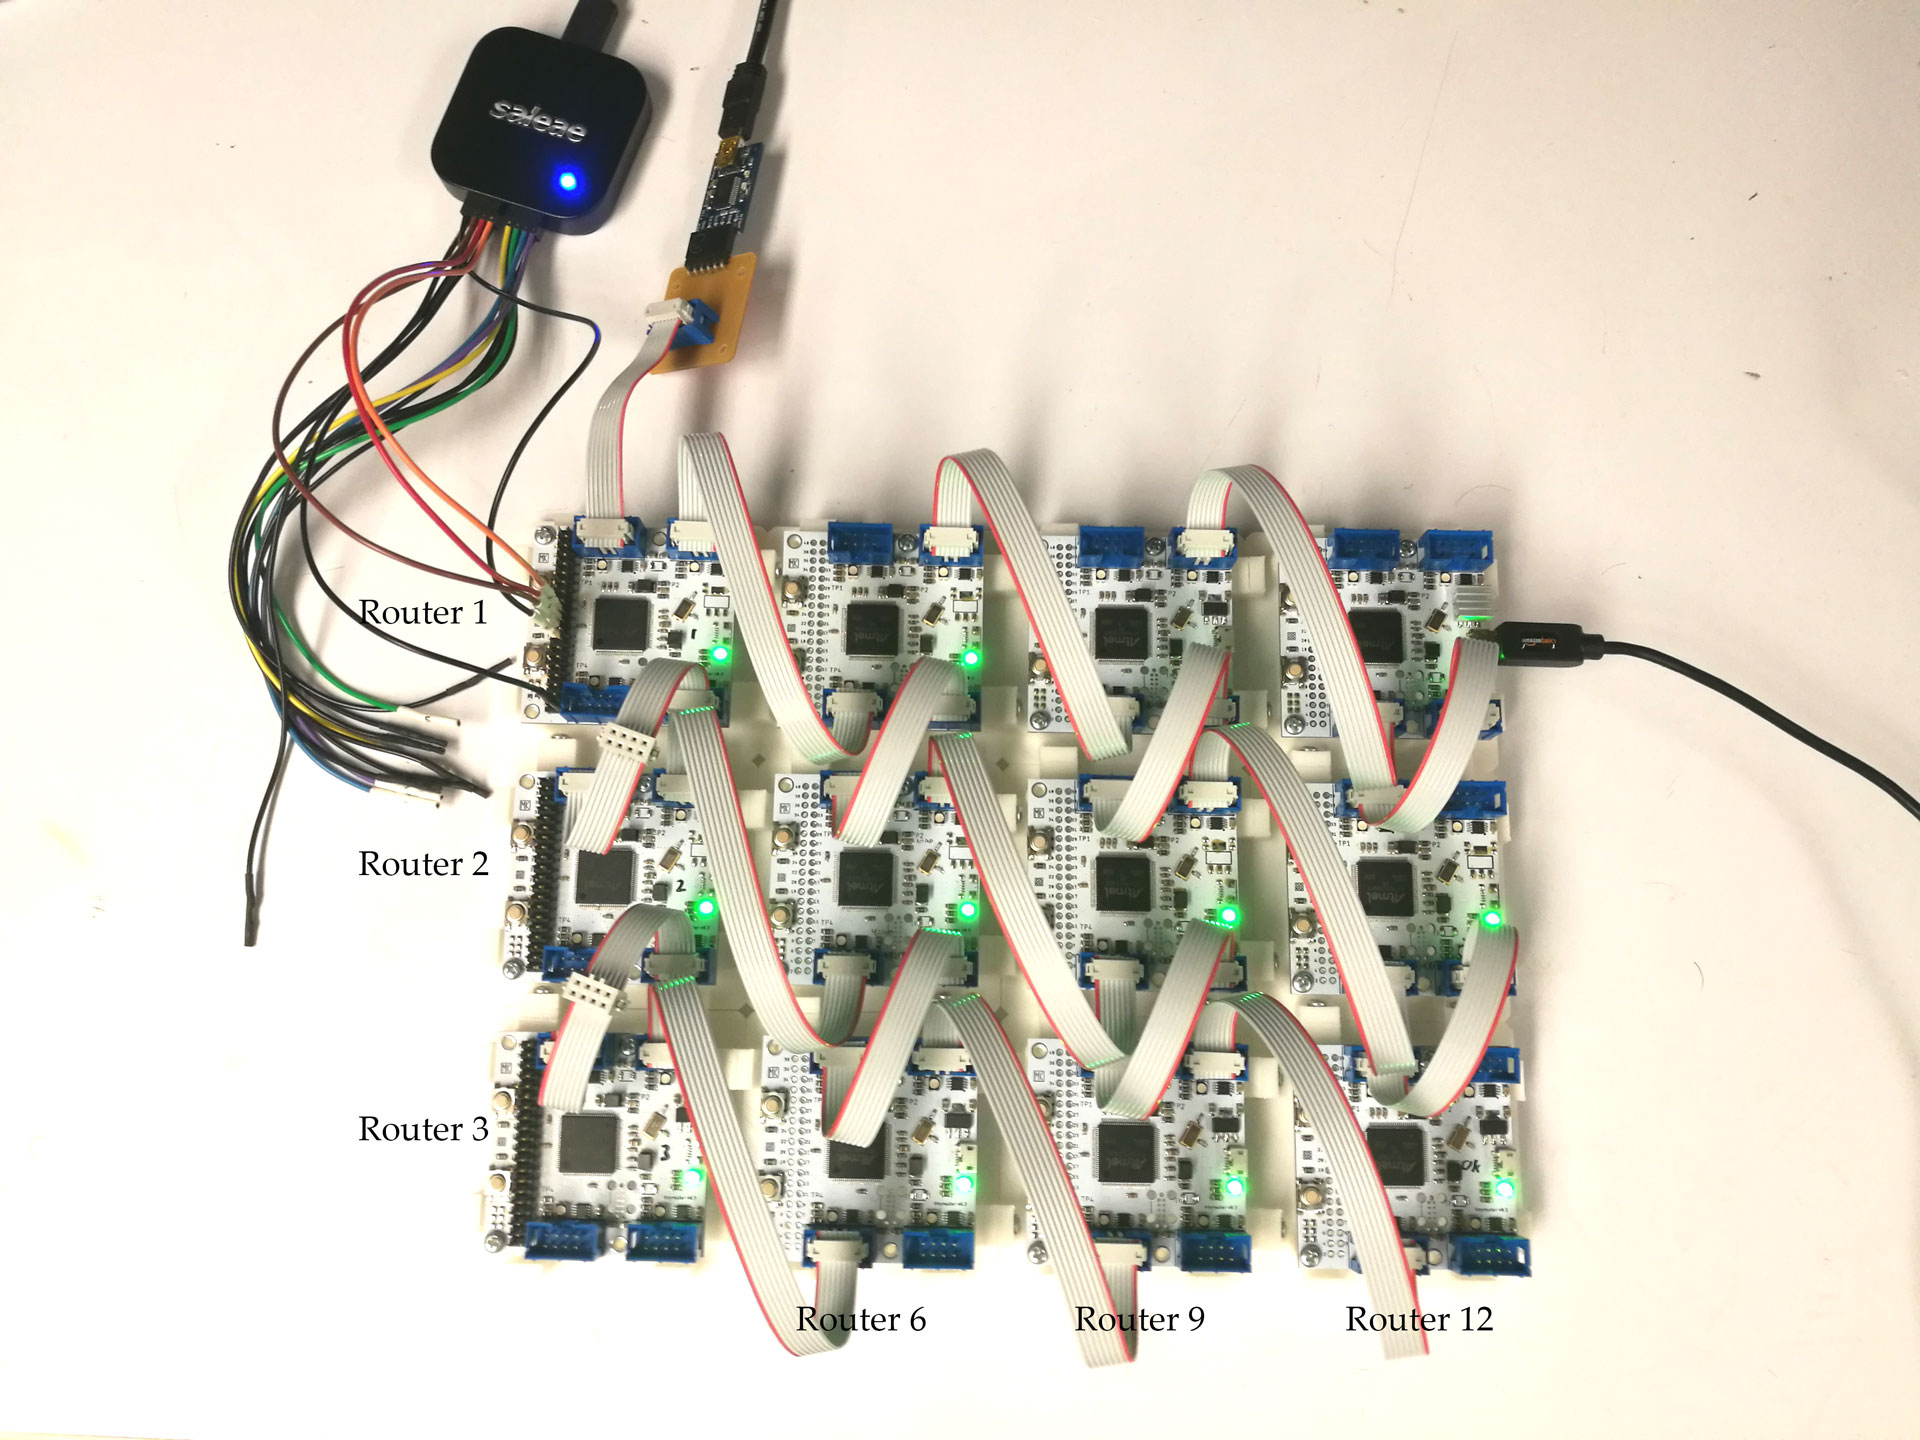
\includegraphics[width=\linewidth]{figures/hardware-12_routers.jpg}
    \caption{The 12-router hardware testbed. Each router is an ATSAMS70-based TinyNet node. The Saleae Logic 8 logic analyzer (left) captures UART timing; the TinyNet Bridge (right, USB) provides host access. Routers are interconnected in a $3\times4$ grid topology.}
    \label{fig:12-routers}
\end{figure}
To assess multi-link routing performance, we assembled a network comprising 12 interconnected TinyNet routers. This setup is illustrated in Fig.~\ref{fig:12-routers}, along with the logic analyzer used for timing Round-Trip Time (RTT) and $\mathrm{D}_{\mathrm{packet}}$ and verifying $\mathrm{L}_{\mathrm{tt}}$. Additionally, a TinyNet Bridge is shown, enabling network access via USB Port. We measured the RTT between Router 1 and Router 12, finding an average RTT of $511\,\mu\mathrm{s}$, captured directly by the logic analyzer and shown in Fig.~\ref{fig:rtt-511us}. This hardware measurement is cross-validated by the simulation result of $505\,\mu\mathrm{s}$ (Section~\ref{sec:sim-val}), a discrepancy of only $1.2\%$, which provides strong corroborating evidence for the accuracy of both measurements.

\begin{figure}[th]
    \centering
    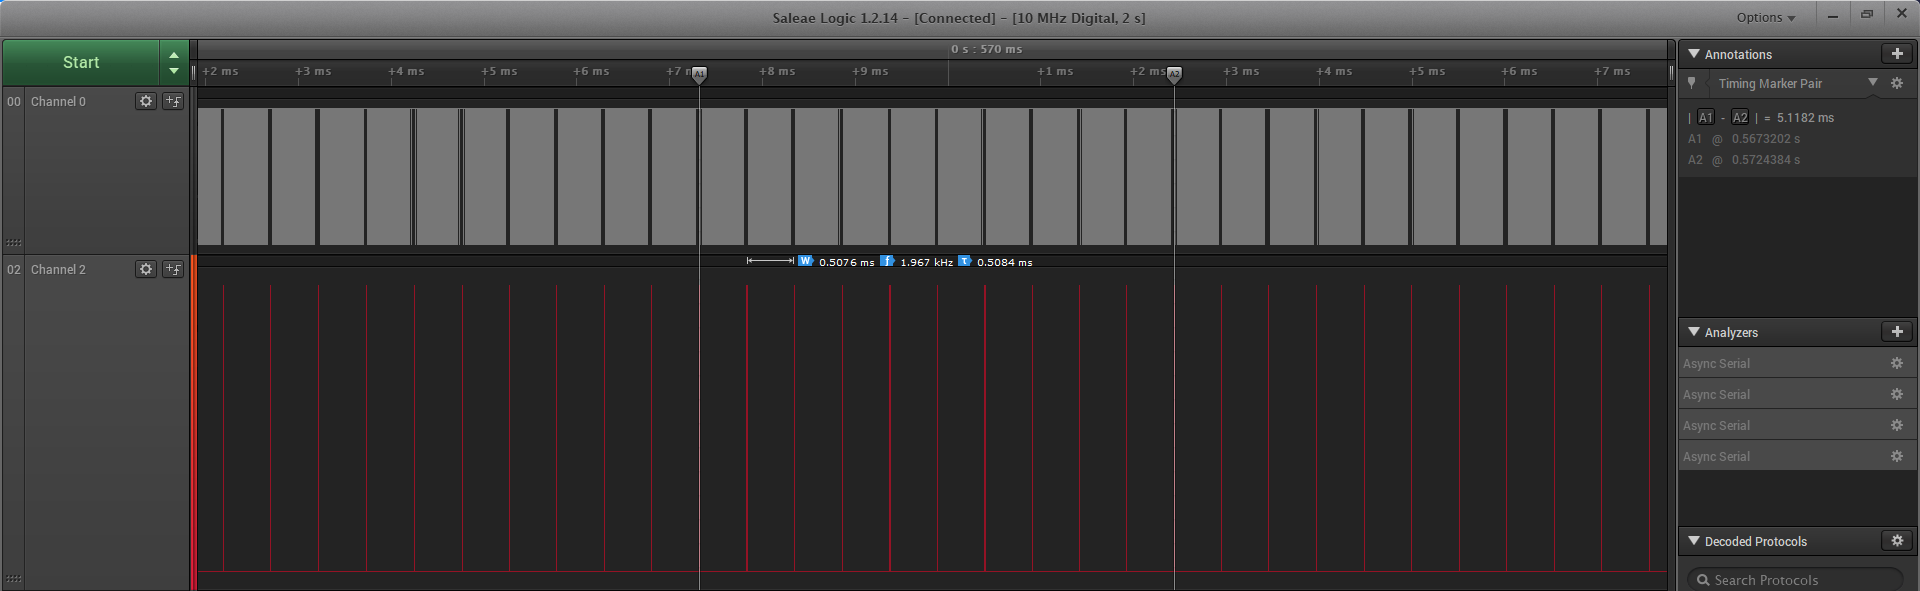
\includegraphics[width=\linewidth]{figures/results-rtt-511us.png}
    \caption{Logic-analyzer capture of the $511\,\mu\mathrm{s}$ round-trip time between Router~1 and Router~12 in the 12-router hardware testbed. The cursors mark the start of the outgoing packet and the end of the returning acknowledgement; this interval is the primary hardware calibration point for the simulation model.}
    \label{fig:rtt-511us}
\end{figure}

\subsection{Simulation Validation}
\label{sec:sim-val}
Our simulation, capable of representing various network topologies and traffic conditions, operates in JavaScript and leverages the open-source Simbit architecture \cite{simbit}. To validate the simulation's effectiveness, we emulate a 12-node grid network, mirroring our hardware setup. We initialize the simulated nodes with parameters derived from hardware measurements via the logic analyzer: processing delay $\mathrm{D}_{\mathrm{process}} = 37\,\mu\mathrm{s}$, per-byte interrupt time $\mathrm{D}_{\mathrm{byte}} = 1.5\,\mu\mathrm{s}$, and link bitrate $\mathrm{L}_{\mathrm{br}} = 20\,\mathrm{MHz}$. All simulations use $\lambda = 0.5$, a heartbeat transmission period of $1\,\mathrm{ms}$, and a missed-heartbeat detection window of $2\,\mathrm{ms}$. This process ensures that our simulation closely resembles real-world hardware operations.

We facilitate message transmission diagonally across the grid and record the round-trip time (RTT). Comparing the RTT of $511\,\mu\mathrm{s}$ obtained from our hardware tests with the simulation's RTT of $505\,\mu\mathrm{s}$, we observe a minor discrepancy of only $1.2\%$, confirming that the simulation accurately reproduces hardware behavior at this operating point. RTT variance and failure-recovery statistics reported in subsequent sections are derived from simulation; hardware validation of these statistics remains future work.

\subsection{Simulation Sensitivity Analysis}
\label{sec:sensitivity}

To bound the effect of hardware timing uncertainty on the reported variance results, we conducted a one-at-a-time sensitivity analysis, independently perturbing each of the three calibrated parameters---$\mathrm{D}_{\mathrm{process}}$, $\mathrm{D}_{\mathrm{byte}}$, and $\mathrm{L}_{\mathrm{br}}$---by $\pm30\%$ from their hardware-measured values and re-running the 10-kHz cross-traffic scenario on the 4$\times$4 grid.

\begin{table}[h]
	\centering
	\caption{Sensitivity of per-hop RTT mean and standard deviation to $\pm30\%$ perturbation of hardware timing parameters. Baseline: $\mathrm{D}_{\mathrm{process}} = 37\,\mu\mathrm{s}$, $\mathrm{D}_{\mathrm{byte}} = 1.25\,\mu\mathrm{s}$, $\mathrm{L}_{\mathrm{br}} = 20\,\mathrm{MHz}$.}
	\label{tab:sensitivity}
	\begin{tabular}{||l|r|r||}
		\hline
		Configuration & Mean ($\mu$s) & $\sigma$ ($\mu$s) \\\hline\hline
		Baseline & 188 & 87 \\
		$\mathrm{D}_{\mathrm{process}} -30\%$ & 53 & 20 \\
		$\mathrm{D}_{\mathrm{process}} +30\%$ & 887 & 392 \\
		$\mathrm{D}_{\mathrm{byte}} -30\%$ & 138 & 56 \\
		$\mathrm{D}_{\mathrm{byte}} +30\%$ & 253 & 98 \\
		$\mathrm{L}_{\mathrm{br}} -30\%$ & 228 & 90 \\
		$\mathrm{L}_{\mathrm{br}} +30\%$ & 217 & 96 \\
		\hline
	\end{tabular}
\end{table}

Bitrate uncertainty has the least influence: a $\pm30\%$ change in $\mathrm{L}_{\mathrm{br}}$ produces at most an 11\% change in $\sigma$. Per-byte interrupt time has moderate influence ($\sigma$ changes $-36\%$ to $+13\%$). Processing delay has the strongest influence: a $+30\%$ perturbation drives the network toward saturation at this traffic level, indicating operation near the processing-capacity boundary.

$\mathrm{D}_{\mathrm{process}}$ is validated by two independent methods: direct logic-analyzer measurement ($37\,\mu\mathrm{s}$) and analytical derivation from the MCU's interrupt service routine (450~cycles $\div$ 300~MHz per-byte, with the forwarding path executing a deterministic instruction sequence). The 1.2\% RTT match at the hardware calibration point confirms this value, bounding the practical uncertainty in $\mathrm{D}_{\mathrm{process}}$ to well under 30\%. The parameters for which the analysis shows benign sensitivity---$\mathrm{D}_{\mathrm{byte}}$ and $\mathrm{L}_{\mathrm{br}}$---are less tightly constrained by independent measurement but do not materially affect the reported results within their plausible uncertainty ranges.

\subsection{Determinism of Communication Time}
A crucial measure of TinyNet's effectiveness is communication time determinism, specifically the standard deviation of the round trip time for each hop a message makes. Different from previous systems that relied on spanning tree models, TinyNet thrives in more extensive network topologies. Therefore, our evaluation focuses on both determinism and robustness within a compact grid setting.

\subsubsection{Evaluation in a 4-by-4 Grid}
\begin{figure}[th]
    \centering
    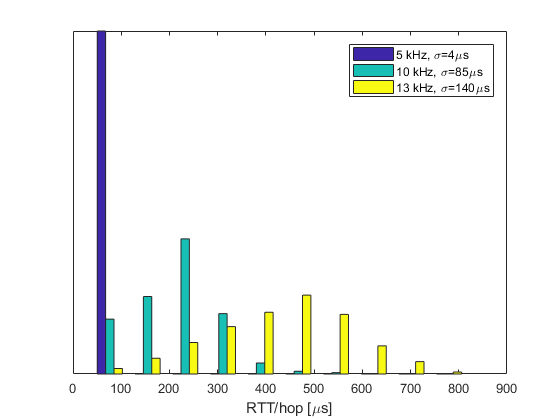
\includegraphics[width=\linewidth]{figures/pdf_grid_cross.png}
    \caption{Per-packet RTT histograms ($x$-axis in $\mu$s) in a 4$\times$4 grid, simulated over 30~ms. Main flow: 5~kHz from node~0 to node~15. Cross-traffic on the opposite diagonal (node~3 to node~12) at 5~kHz (top), 10~kHz (middle), and 13~kHz (bottom). Standard deviations: $\sigma = 4$, 85, and $140\,\mu\mathrm{s}$, respectively.}
    \label{fig:hists-cross}
\end{figure}
We begin by simulating a 4-by-4 grid of nodes, with each node having a packet delay time of $37 \mu \mathrm{s}$ (the hardware-measured $\mathrm{D}_{\mathrm{process}}$) and each link operating at a bitrate of 20 MHz. We transmit crucial messages diagonally across the grid at 5 kHz for 30 ms. Simultaneously, we model varying levels of cross-traffic on the opposite diagonal: 5 kHz, 10 kHz, and 13 kHz in separate simulations. The resulting histograms of per-packet round trip times are shown in Fig.~\ref{fig:hists-cross}, with standard deviations of $4 \mu \mathrm{s}$, $85 \mu \mathrm{s}$, and $140 \mu \mathrm{s}$ for each traffic scenario, respectively.

\subsubsection{Evaluation in a Simulated Airplane Wing Network}
\begin{figure}[th]
    \centering
    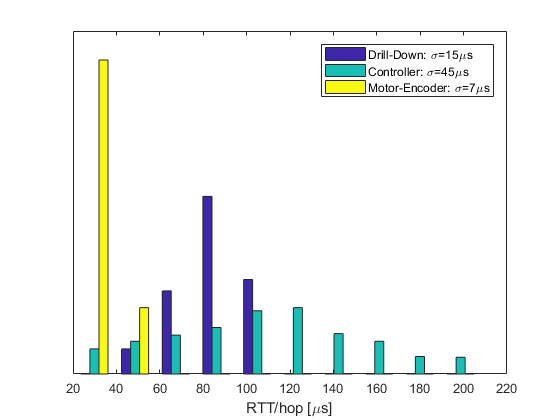
\includegraphics[width=\linewidth]{figures/pdf_RTT.png}
    \caption{Per-hop RTT histograms ($x$-axis in $\mu$s) in a simulated airplane wing topology: one master node, three controllers, 24 motors, and 24 encoders, simulated over 30~ms. Standard deviations: master--encoder queries $\sigma = 15\,\mu\mathrm{s}$, controller--motor loops $\sigma = 45\,\mu\mathrm{s}$, motor--encoder loops $\sigma = 7\,\mu\mathrm{s}$.}
    \label{fig:hists-airplane}
\end{figure}
In addition, we assess determinism within a simulated airplane wing network, structured into four layers: a single master node on top, three controllers in the second layer, each connected to eight motors in the third layer, and each motor linked to two neighboring motors and an encoder in the fourth layer. Under the same hardware parameters as the grid, the motors maintain a 2.5-kHz control loop with their encoders, the controllers manage a 1-kHz loop with each motor, and the master node queries each encoder at 500 Hz. This simulation, conducted over 30 ms, reveals per-hop round trip times as illustrated in Fig.~\ref{fig:hists-airplane}, with a standard deviation of $15 \mu \mathrm{s}$ for master-encoder queries, $45 \mu \mathrm{s}$ for controller-motor loops, and $7 \mu \mathrm{s}$ for motor-encoder loops.

These results highlight two key outcomes:
\begin{itemize}
    \item \textbf{Impact of Network Traffic on Determinism:} An increase in network traffic tends to reduce network determinism. As the number of packets traversing the network grows, so does the buffer depth at individual nodes, leading to increased message latency and variability in latency. This relationship is compounded by path length: networks with more routing hops expose each packet to more opportunities for queuing, so determinism degrades faster per unit of added traffic in larger networks. This is consistent with the airplane wing results, where the short motor-encoder paths (few hops) achieve $\sigma = 7\,\mu\mathrm{s}$ while the longer master-encoder paths (many hops) exhibit $\sigma = 15\,\mu\mathrm{s}$ under similar per-link traffic loads.
    \item \textbf{TinyNet's Adaptability:} Despite the challenges of heavy cross-traffic, TinyNet maintains a high level of message determinism. Its dynamic adaptation to changing traffic conditions across different network areas effectively distributes the load among numerous nodes. This approach not only reduces message delivery time but also helps in consistently maintaining low latency levels.
\end{itemize}

\subsection{Robustness to Node Failure}
\label{sec:robustness}
\begin{figure}[th]
    \centering
    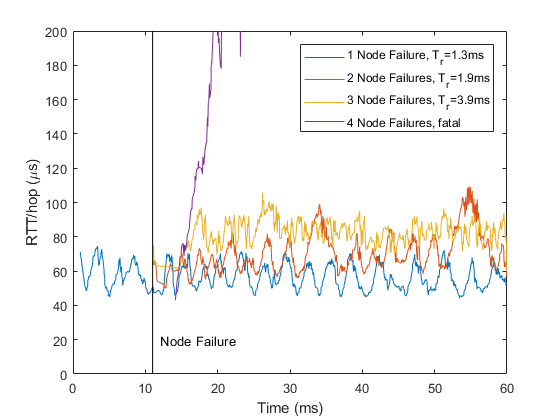
\includegraphics[width=\linewidth]{figures/node_failure_recovery.png}
    \caption{Per-packet RTT ($y$-axis in $\mu$s, $x$-axis in ms over 0--30~ms window) in the 4$\times$4 grid before and after random interior node removal at $t=11\,\mathrm{ms}$. Colors denote failure count: 1~node (blue), 2~nodes (orange), 3~nodes (green), 4~nodes (red). Recovery times (RTT returning to within $2\times$ pre-failure mean): 1.3~ms, 1.9~ms, and 3.9~ms for 1, 2, and 3 node failures, respectively. Four-node removal (25\%) did not converge within the simulation window.}
    \label{fig:failure}
\end{figure}
Robustness to node failure is the second crucial dimension of TinyNet's performance, focusing on the network's ability to rapidly respond to and recover from node failures. For assessing this essential aspect, we conducted simulations on a 4-by-4 grid of nodes, using the same hardware parameters as in our message determinism evaluation. In these simulations, corner nodes sent messages diagonally across the grid at frequencies of 10 kHz and 5 kHz. At 11 milliseconds into the simulation, we randomly disconnected one, two, three, or four nodes simultaneously (chosen uniformly at random from the interior nodes of the grid), then observed and recorded the subsequent message delay times. Each failure-count condition was repeated across multiple independent trials with different randomly selected node sets, and the reported recovery times represent the average across those trials. Recovery is defined as the point at which the per-packet delay returns to within $2\times$ of its pre-failure mean. The findings, depicted in Fig.~\ref{fig:failure}, show per-packet delay over time with the failure event at $t = 11\,\mathrm{ms}$. After a single node failure, the network recovered in 1.3 ms; after two failures, in 1.9 ms; and after three failures, in 3.9 ms.

Key observations from these results include:
\begin{itemize}
    \item \textbf{Rapid Recovery from Failures:} TinyNet recovers from node failures within 1.3--3.9~ms. Even with approximately 19\% of the network (3 of 16 nodes) failing simultaneously, TinyNet maintains round trip times effectively. By contrast, the stateful LFA baseline drops approximately 250 packets during the 50~ms BFD cutover window before routing resumes (see Section~\ref{sec:comparison}).
    \item \textbf{Impact of Multiple Node Failures:} The loss of a single node does not significantly affect long-term communication. However, multiple node failures can adversely affect both message latency and network determinism. This outcome is predictable as TinyNet's load-balancing capabilities are most effective when there are sufficient alternative nodes for message rerouting.
    \item \textbf{Capacity for Message Maintenance in Failures:} TinyNet sustains message transmission even under substantial network failures. In contrast to spanning-tree protocols, which lose connectivity to entire sub-trees on a single node failure~\cite{spb}, TinyNet reroutes around failed nodes by flooding. However, recovery did not converge within the simulation window at a 25\% failure rate (4 of 16 nodes simultaneously), indicating that sufficient path redundancy is a prerequisite for TinyNet's rerouting to succeed.
\end{itemize}

\subsection{Comparison Against a Stateful Routing Baseline}
\label{sec:comparison}
\begin{figure}[th]
    \centering
    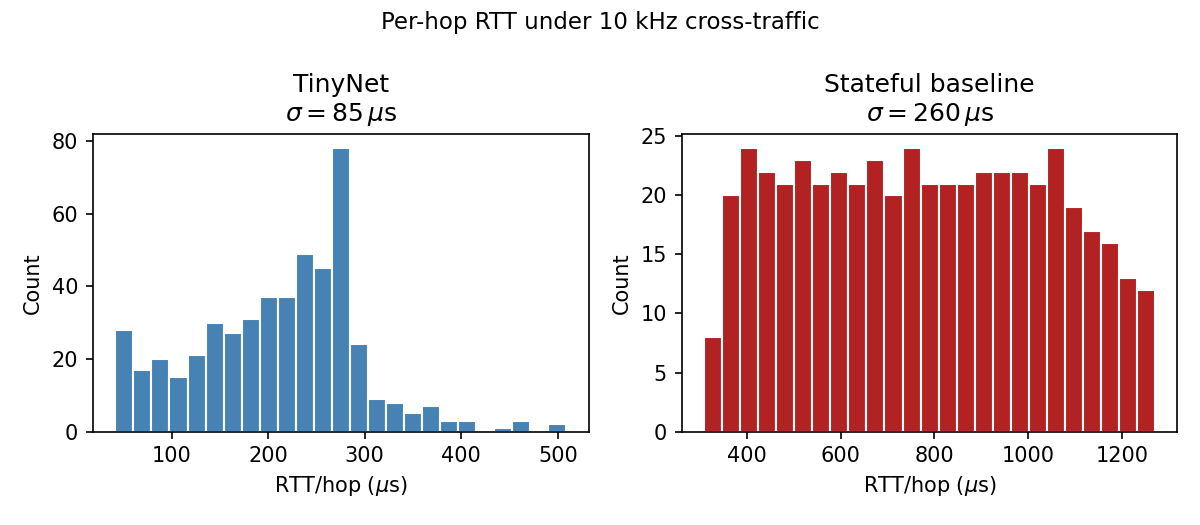
\includegraphics[width=\linewidth]{figures/comparison_cross.png}
    \caption{Per-hop RTT histograms ($x$-axis in $\mu$s) under 10~kHz cross-traffic on the 4$\times$4 grid: TinyNet (left, $\sigma = 85\,\mu\mathrm{s}$) versus stateful shortest-path baseline (right, $\sigma = 139\,\mu\mathrm{s}$), a 39\% reduction in variability.}
    \label{fig:comparison-cross}
\end{figure}
\begin{figure}[th]
    \centering
    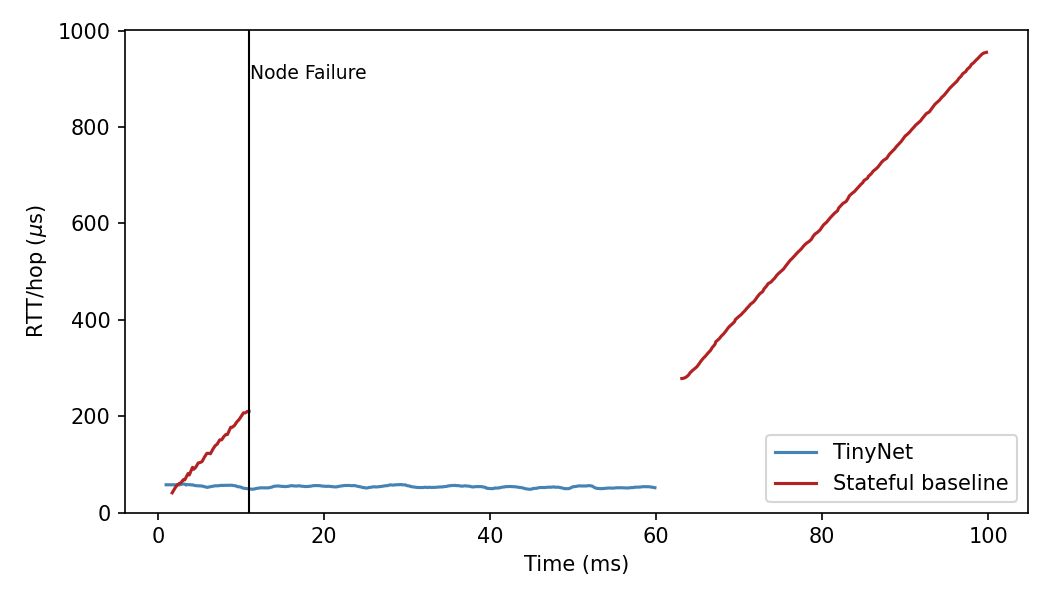
\includegraphics[width=\linewidth]{figures/comparison_failure.png}
    \caption{Cumulative packets delivered ($y$-axis, 0--30~ms window on $x$-axis) following a single interior node failure at $t=11\,\mathrm{ms}$: TinyNet (blue) versus LFA-style stateful baseline (red). Both lines overlap before the failure. TinyNet misses fewer than 20 packets and recovers in $\approx\!3\,\mathrm{ms}$; the baseline's 50~ms flat segment (packets dropped during BFD detection and LFA cutover) represents $\approx\!250$ undelivered packets.}
    \label{fig:comparison-failure}
\end{figure}

To directly address the question of how TinyNet compares against stateful routing, we implemented a shortest-path baseline in our JavaScript simulator. The baseline pre-computes BFS shortest paths at startup and routes each packet along the single lowest-hop-count path, with no multipath. On link failure, it drops all packets destined for affected nodes for 50\,ms---the typical BFD detection plus LFA switchover window \cite{rfc5286,cisco_lfa}, and the current best-case for stateful IP Fast Reroute (see Section~\ref{sec:related:frr})---before recomputing routes. We compare against LFA rather than RPL because LFA represents the fastest-recovering class of stateful protocols in production use; RPL's DODAG repair mechanism targets energy-constrained wireless links and operates on a fundamentally different latency regime not directly applicable to UART-connected NCS (see Section~\ref{sec:related:mesh}).

\subsubsection{RTT Determinism Under Cross-Traffic}
Fig.~\ref{fig:comparison-cross} shows per-hop RTT histograms under 10 kHz cross-traffic for both protocols on the same 4-by-4 grid. TinyNet achieves a standard deviation of $85\,\mu\mathrm{s}$, compared to $139\,\mu\mathrm{s}$ for the stateful baseline---a $39\%$ reduction in variability. The improvement stems from TinyNet's cost function actively redistributing packets across multiple paths in response to buffer occupancy, whereas the stateful baseline funnels all traffic through a single fixed path, allowing congestion to build without relief.

\subsubsection{Failure Recovery}
Fig.~\ref{fig:comparison-failure} shows cumulative packets delivered following a single node failure at $t=11\,\mathrm{ms}$. Before the failure both protocols deliver at the same rate; the lines overlap. After the failure, TinyNet recovers in approximately 3\,ms as packets immediately flood to alternate paths, missing fewer than 20 packets in total. (The 1.3\,ms single-failure figure reported in Section~\ref{sec:robustness} is measured by a different metric---per-packet RTT returning to within $2\times$ of its pre-failure mean---under dual diagonal traffic at 10\,kHz plus 5\,kHz; the 3\,ms figure here is read from the cumulative delivery curve under 5\,kHz single-diagonal traffic and therefore reflects a different saturation point.) The stateful baseline's cumulative count is flat for 50\,ms---the LFA detection and cutover window \cite{rfc5286,cisco_lfa}---before routing resumes; this 50\,ms flat segment is the expected, designed behavior of LFA: during BFD timeout, packets destined for the failed path are dropped, and the baseline does not resume delivery until the cutover completes. This flat segment represents approximately 250 undelivered packets. This more-than-order-of-magnitude difference in recovery time (3\,ms vs.\ 50\,ms) reflects the fundamental asymmetry between TinyNet's data-driven reroute and LFA's pre-computed backup activation: TinyNet's first post-failure packet triggers flooding immediately, while LFA must wait for BFD to time out before switching to its pre-installed alternate.
\section{Conclusion}
This paper introduces TinyNet, a novel routing protocol tailored for Networked Control Systems, emphasizing Message Delivery Time Determinism over Total Throughput. TinyNet's efficacy in routing messages using minimalistic hardware has been showcased alongside a simulation tool that assesses its performance. A standout feature of TinyNet is its ability to manage message routing in extensively connected networks without relying on a Network Controller or requiring nodes to possess complete network topology knowledge.

The pivotal contribution of this work is the creation of a port-forwarding strategy that utilizes real-time data about queue sizes at subsequent hops. This innovation allows for the intelligent rerouting of packets to circumvent congested network segments.

Determining realistic usage profiles for Network Control Systems has been challenging due to limited existing research. We plan to gather primary data on practical applications and challenges in this field by consulting industry stakeholders at companies like Boeing, Airbus, Kittyhawk, and Moog Inc.

The use of UART presents limitations in our project, specifically in capping the permissible bitrate to only 3.125 Mbps and necessitating a ``stateful'' environment where all ports must share the same baudrate settings. To address these issues, one future direction could include an FPGA-based link layer, implementing a ``co-clocking'' technique for establishing bitrate. In this approach, neither side of a transmission pre-defines a bitrate. Instead, data transfer occurs in a responsive manner: once one side shifts data into a register, it sends an acknowledgment bit, triggering the transmission of the next bit. This method has successfully achieved bitrates of up to 65 Mbps. We have integrated this system with a microcontroller analogous to the ATSAMS70 used in the TinyNet router, achieving similar transmission speeds via a 5-MHz wide parallel bus. This advancement aims to establish a completely stateless, configuration-free system, significantly enhancing the flexibility and scalability of TinyNet's network infrastructure.

In addition to leveraging FPGAs for a stateless link layer, FPGAs can also be used for switching and port-forwarding, leveraging the simplicity of the TinyNet protocol for implementation in Verilog. This effort is expected to surpass the performance of Switched Ethernet while preserving the stateless, fault-tolerant, and adaptive qualities of TinyNet.

Finally, the current routing protocol employs a lambda function, as outlined in equation (\ref{eq:cost}), for navigating around busy ports. We aim to explore machine learning techniques to refine this function, optimizing the routing process based on network topology and cost considerations, thereby enhancing overall network performance.
\section*{Declaration of Generative AI and AI-assisted Technologies in the Writing Process}
During the preparation of this work the authors used GPT4 in order to improve readability. After using this tool, the authors reviewed and edited the content as needed and take full responsibility for the content of the publication.

\begin{ack}
	This research has received no external funding.
\end{ack}

\bibliographystyle{plain}
\bibliography{root}

\newpage
\section*{Appendix}
\renewcommand{\thefigure}{A.\arabic{figure}}
\setcounter{figure}{0}
\begin{figure*}[th]
	\centering
	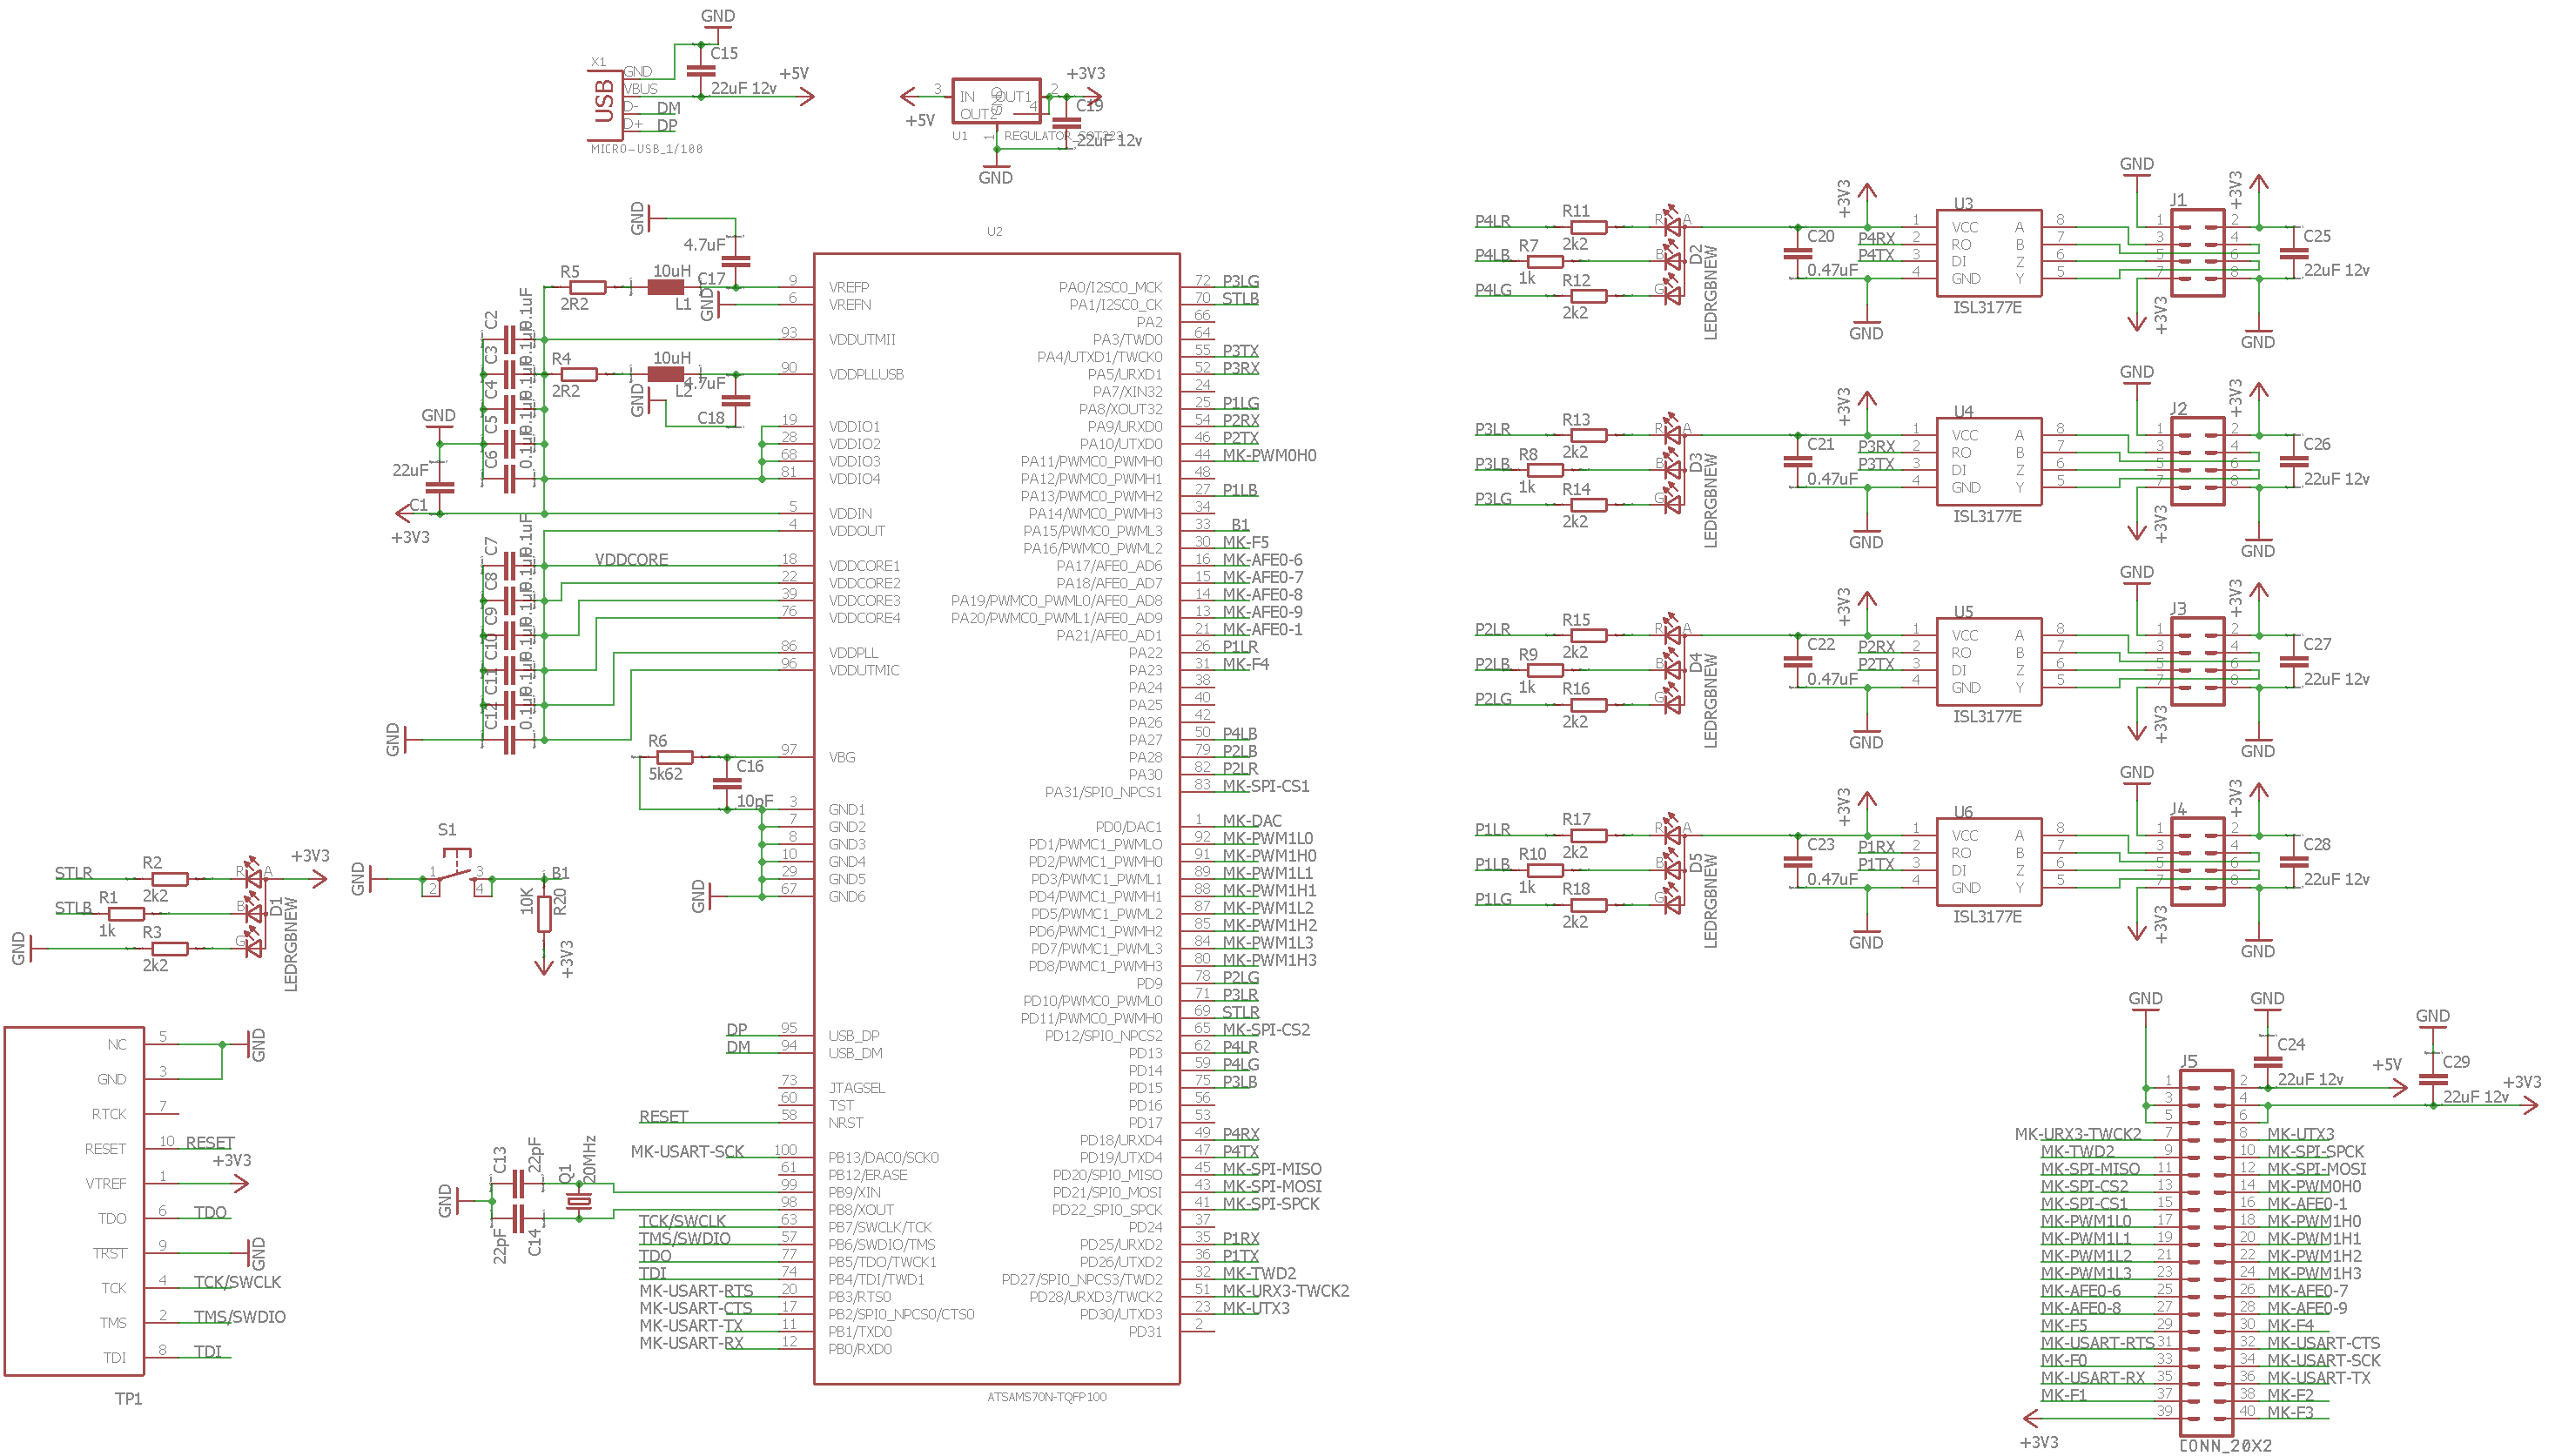
\includegraphics[width=\textwidth]{figures/atsam-router-schematic.png}
	\caption{ATSAMS70-based TinyNet router schematic. Each UART port connects to an ISL3177E differential line driver for RS-485-compatible signaling. Port-select logic and buffer management run on the 300~MHz core.}
	\label{fig:router-schematic}
\end{figure*}
\begin{figure*}[th]
	\centering
	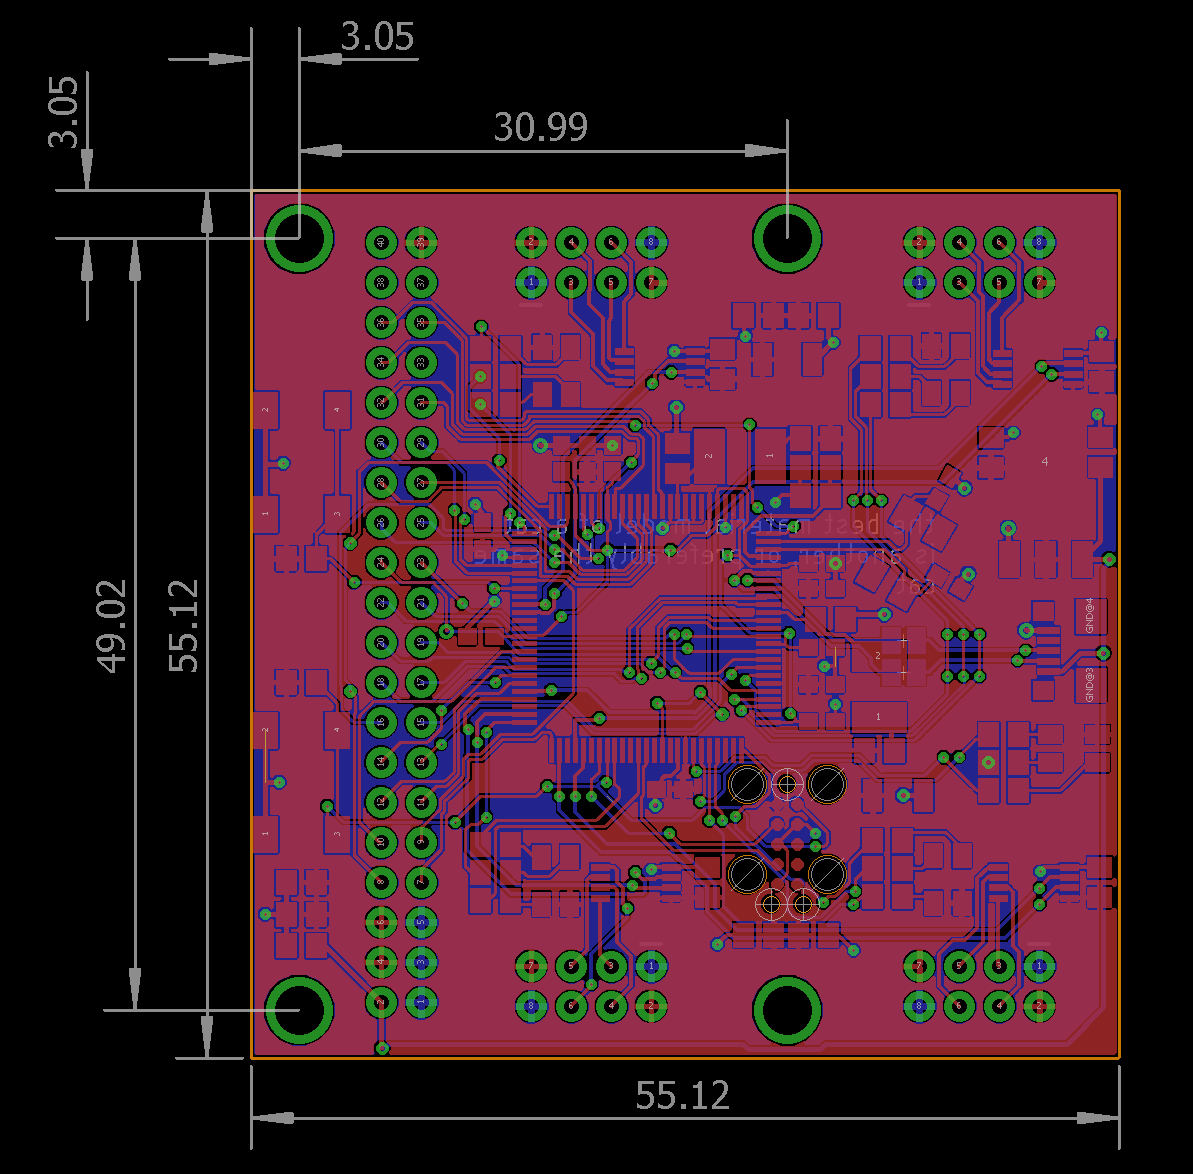
\includegraphics[width=\textwidth]{figures/atsam-router-board.png}
	\caption{TinyNet router PCB layout. The ATSAMS70 microcontroller occupies the center; ISL3177E drivers are arranged at the board periphery, one per UART port.}
	\label{fig:router-board-file}
\end{figure*}

\end{document}